\chapter{Metadata}
\label{txt:metadata}
\index{Metadata|(}
Metadata is `data about data'. In Corina this means all the information associated with your physical samples and measurement series e.g. species, location, who measured it, dimensions, slope, soil type etc.

The metadata in Corina, and in fact the entire Corina data model, is based on the Tree Ring Data Standard (TRiDaS). Before you use Corina you may find it useful to read \citet{tridas} so that you get a better understanding of the principles of TRiDaS, but a summary is also provided here.

\section{Tree Ring Data Standard - TRiDaS}
\index{TRiDaS|textbf}
TRiDaS is an XML-based data standard for recording dendrochronological data and metadata. More than 80 dendrochronologists, computer scientists and specialists from research disciplines that rely on dendrochronology have so far contributed to its development, including dendroarchaeologists, art and architecture historians, ecologists, geologists and climatologists.  The standard is therefore capable of recording the wide variety of metadata required by these different fields. TRiDaS builds upon other established standards, such as GML for the recording of locality information.  The extensible nature of XML also means that TRiDaS can evolve to accommodate the changing needs of dendrochronologists over time.  

TRiDaS includes a total of eight data entities: project; object; element; sample; radius; measurementSeries; derivedSeries; and value.  Detailed descriptions of each of these entities are given below and their relationships are illustrated in figure \ref{fig:datamodel}.

\begin{figure}
\centering
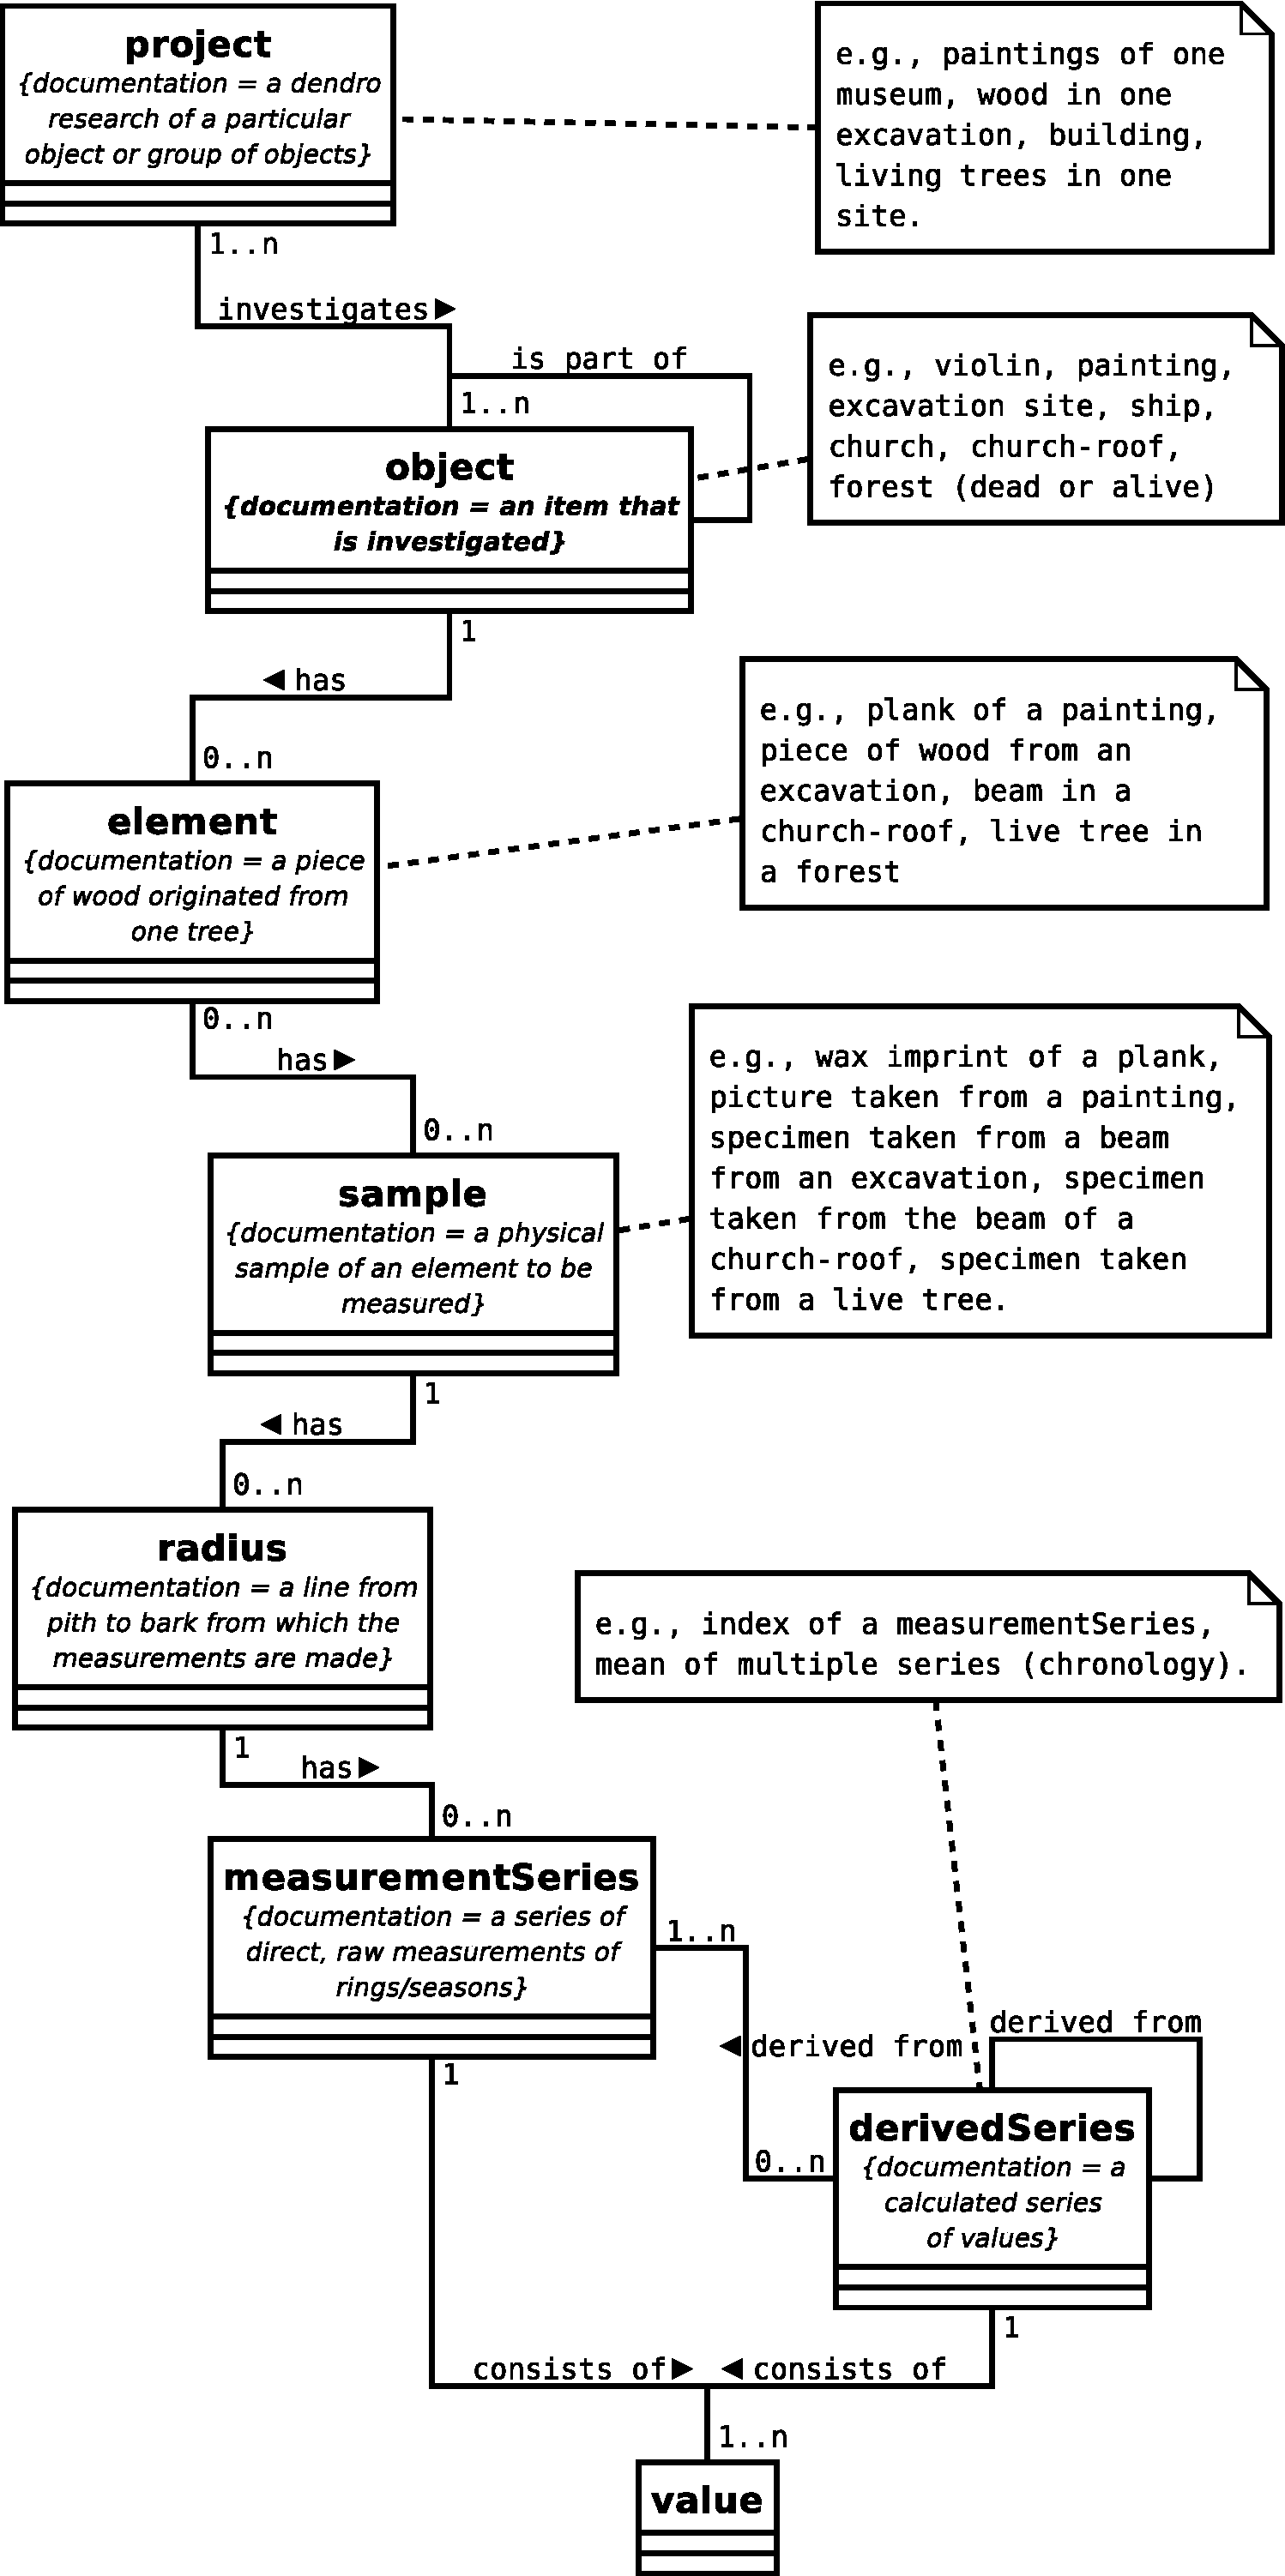
\includegraphics[height=0.9\textheight]{Images/datamodel.pdf}
\caption{TRiDaS data model showing the relationships between data entities.  Most of the entities having a simple hierarchical relationship (a project has one or more objects, an element has one or more samples.} 
\label{fig:datamodel}
\end{figure}

\begin{description}

\item 
\includegraphics[width=5mm]{Images/pixel.png}  \textbf{A project} -- is defined by a laboratory and encompasses dendrochronological research of a particular object or group of objects.  Examples include: the dating of a building; the research of forest dynamics in a stand of living trees; the dating of all Rembrandt paintings in a museum. What is considered a ``project'' is up to the laboratory performing the research. It could be the dating of a group of objects, but the laboratory can also decide to define a separate project for each object. Therefore, a project can have one or more objects associated with it.  Due to the way research is conducted at the Cornell Tree-Ring Lab, TRiDaS projects are not currently supported within Corina, although future plans include adding project support.

\item 
\includegraphics[width=5mm]{../src/edu/cornell/dendro/corina_resources/Icons/128x128/object.png} \textbf{An object} -- is the item to be investigated.  Examples include: violin; excavation site; painting on a wooden panel; water well; church; carving; ship; forest. An object could also be more specific, for example: mast of a ship; roof of a church. Depending on the object type various descriptions are made possible. An object can have one or more elements and can also refer to another (sub) object.  For instance a single file may contain three objects: an archaeological site object, within which there is a building object, within which there is a beam object.  The list of possible object types is extensible and is thus flexible enough to incorporate the diversity of data required by the dendro community.  Only information that is essential for dendrochronological research is recorded here. Other related data may be provided in the form of a link to an external database such as a museum catalogue. 

\item 
\includegraphics[width=5mm]{../src/edu/cornell/dendro/corina_resources/Icons/48x48/element.png} \textbf{An element} -- is a piece of wood originating from a single tree. Examples include: one plank of a water well; a single wooden panel in a painting; the left-hand back plate of a violin; one beam in a roof; a tree trunk preserved in the soil; a living tree. The element is a specific part of exactly one object or sub object.  An object will often consist of more than one element, e.g., when dealing with the staves (elements) of a barrel (object).  One or more samples can be taken from an element and an element may be dated using one or more derivedSeries.

\item 
\includegraphics[width=5mm]{../src/edu/cornell/dendro/corina_resources/Icons/48x48/sample.png} \textbf{A sample} -- is a physical specimen or non-physical representation of an element. Examples include: core from a living tree; core from a rafter in a church roof; piece of charcoal from an archaeological trench; slice from a pile used in a pile foundation; wax imprint of the outer end of a plank; photo of a back plate of a string instrument. Note that a sample always exists and that it can either be physical (e.g.\ a core) or representative (e.g.\ a picture). A sample is taken from exactly one element and can be represented by one or more radii.

\item 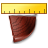
\includegraphics[width=5mm]{../src/edu/cornell/dendro/corina_resources/Icons/48x48/radius.png} \textbf{A radius} --  is a line from pith to bark along which the measurements are taken. A radius is derived from exactly one sample. It can be measured more than once resulting in multiple measurementSeries.

\item 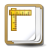
\includegraphics[width=5mm]{../src/edu/cornell/dendro/corina_resources/Icons/48x48/measurementseries.png} \textbf{A measurementSeries} -- is a series of direct, raw measurements along a radius. A single measurementSeries can be standardised or a collection of measurementSeries can be combined into a derivedSeries.  The measurements themselves are stored separately as values.

\item 
\includegraphics[width=5mm]{../src/edu/cornell/dendro/corina_resources/Icons/48x48/derivedseries.png} \textbf{A derivedSeries} -- is a calculated series of values and is a minor modification of the ``v-series'' concept proposed by \cite{corina}.  Examples include: index; average of a collection of measurementSeries such as a chronology. A derivedSeries is derived from one or more measurementSeries and has multiple values associated with it.

\item 
\includegraphics[width=5mm]{Images/pixel.png} \textbf{A value} --  is the result of a single ring measurement. Examples include: total ring width; earlywood width; latewood width. The values are related to a measurementSeries or a derivedSeries. In case of a measurementSeries the variable and its measurement unit (e.g.\ microns, 1/100th mm etc) are recorded as well.  Corina currently only supports total ring width values.  Support for other variables is planned for a future version.

\end{description}


Working top to bottom, the TRiDaS entities are nested within each other.  For instance a project contains one or more objects, which in turn contains one or more elements, and so on.  The benefit of this is that you record data once and once only.  In standard file-based dendrochronological software, when creating measurement series you are typically required to type the name of the site, the species of tree etc over and over again.  This is not only time consuming, but very error prone.  

Keeping data consistent is also difficult.  For instance, if it was determined that a tree species was identified incorrectly, in existing file-based software, the user would need to locate all data series from this tree and manally update the metdata.  This is not the case in Corina.  A tree is represented just once in Corina and samples of this tree, and the subsequent measurement series reference this one entry.  If metadata for this tree needs to be changed, the tree record is updated in just this one place.  Because the measurement series obtain this information by reference, then all associated series are automatically kept up to date.

\section{Entering sample metadata}
\index{Sample!Metadata, editing}
\index{Metadata!Editing}
The metadata for a series is viewed and edited on the `Metadata' tab of the main window such as that shown in figure \ref{fig:metadata}.  You can see the interface is organized according to the TRiDaS data model with separate screens for object, through to series.  

\begin{figure}
\centering
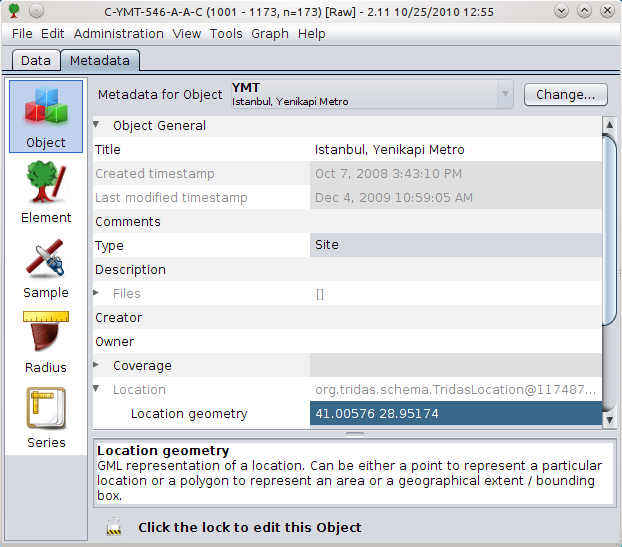
\includegraphics[width=0.6\textwidth]{Images/metadata.png}
\caption{Example of the metadata dialog.  The screen is showing the details of a TRiDaS object.  Note that the location geometry field is highlighted and so a description of what is expected in this field is given below.} 
\label{fig:metadata}
\end{figure}

When creating a new series, the metadata screens must be populated in order.  This is necessary because of the nesting of entities described above.  For instance, an element is associated with an object, so an object must be chosen because and element can be defined.  Likewise, an element must be chosen before any samples of this element can be defined.  

Much of the time the entities that you need will already be stored within the database.  Instead of re-entering data, you simply need to select the existing entry from the database, saving a great deal of time.  Depending on the situation buttons will appear at the top of the dialog to let you `choose' an entry from the database, `revert' to the previously chosen entry, `change' the existing entry to a different one from the database, or create a `new' record.

Please note that the content of these metadata screens is kept read-only by default.  To edit the values, you must first click the padlock icon to unlock the fields.  When you have finished making changes you need to press the save button to write the changes to the database before moving to another metadata screen.

Very few of the metadata fields in the TRiDaS data model are mandatory, but a few are.  In this case, these fields are highlighted with a red background.  Note that whether a field is mandatory or not can depend on the other fields that have been filled in.  For instance, the dimensions of an element are not required, but if dimensions are given then the units for these measurements must also be provided.

A number of the metadata fields are restricted with regards the values that you can enter.  These are known as `controlled vocabularies' in TRiDaS terms.  Controlled vocabulary fields are represented by drop down menus.  Similarly fields that expect numerical values (such as element dimensions) will only allow numbers.  The final method data entry method is through custom dialogs.  The only custom dialog currently implemented is for locations.  This accepts coordinates in either decimal degrees or degrees minutes and seconds.  Alternatively you can use data from a GPS handset by providing a GPS Exchange (GPX) format file containing the waypoints. The GPX format is the most common interchange format for GPS data. You can pick the relevant waypoint from the drop down menu.  You can also preview the defined coordinates on a map using the `view on map' button. 

\tip{A popular open source GPS communication tool is GPS Babel.  It is an easy to use application which can download data from the majority of GPS handsets.  See \url{http://www.gpsbabel.org} for more information.}


\section{Entering bulk metadata}
\index{Metadata!Bulk entry}
\label{txt:bulkentry}
Entering metadata on a sample-by-sample basis works perfectly well, but does not necessarily fit best with the typical workflow of a laboratory.  Samples do not typically arrive in a lab in ones and twos, rather in large quantities following a field excursion.  In this case it is most efficient to enter all the metadata for the samples as they arrive.  This is often best in terms of data accuracy as the metadata can be entered while the field notes are still fresh in the mind.

To enable the efficient entry of lots of metadata Corina includes the bulk data entry interface.  This can be access from the file menu and is illustrated in figure \ref{fig:bulkentry}.  There are three pages, one each for objects, elements and samples.

\begin{figure}
\centering
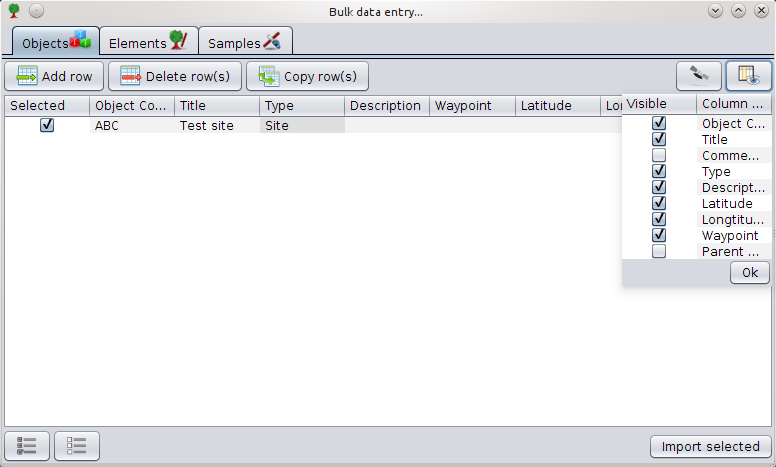
\includegraphics[width=0.6\textwidth]{Images/bulkentry.png}
\caption{The bulk metadata entry screen.  The `show/hide columns' button has been pressed showing how the user can turn on and off particular columns.} 
\label{fig:bulkentry}
\end{figure}

The interface is designed like a spreadsheet so as to be as familiar to users as possible.  Each row of the table represents a new entry in the Corina database.  Which columns are shown to the user is determined by the `show/hide columns' button on the top right of the screen.  

The bulk entry interface also includes support for reading GPS units.  By pressing the satellite button on the toolbar, the user can provide a GPS Exchange (GPX) format file containing the waypoint locations recorded in the field.   Corina will add a waypoint column to the spreadsheet with a drop down menu which will automatically populate the latitude and longitude fields for the record. 

It is common for many of the metadata fields to be same in a single field collection.  For instance, when coring trees in a forest, they are often of the same species.  Rather than requiring the user to repeatedly type the same data over and over, the `copy row' button can be used to duplicate a record, and then the user can change the few fields that are different.

When you have entered all the data you want, you can press the `Import selected' button to write the records to the database.  

\section{Metadata browser}
\index{Metadata!Browsing}
The metadata browser interface provides a convenient way to view all the metadata within your Corina database.  It can be accessed through the `Administration' menu.

The metadata browser contains two parts: a hierarchical representation of all TRiDaS entities in your database on the left; and a metadata viewer for the selected entry on the right.  This interface is also the best method for fixing mistakes in your database.  

Although Corina's database architecture maintains integrity within your data, it does come at the price of being a little more complicated to fix mislabelled series.  For instance, what if you were to measure a series 'B' and assign it to sample ABC-138-A only later to realize you misread the label and it was in fact ABC-188-A.  In a traditional file-based system, you would probably just need to rename the file you'd just created.  In Corina however, you need to redefine the relationship of the series within the database and reassign it to the create sample.  This is best understood when looking at the hierarchical tree in the metadata browser.  Hopefully you will see that you what you need to do is to move the series from its current position in the database to the correct one.  

The reorganization of data in this way is achieved by right clicking on items in the hierarchical tree and choosing with `merge' or `reassign'.
%% TODO - Finish


\section{Laboratory codes}
\index{Laboratory codes}
\index{Sample codes|see{Laboratory codes}}
Corina uses lab codes to refer to the hierarchical nature of the TRiDaS entities in the database.  The separate parts of the code a delimited by hyphens and depending on the level of the entity you are referring to, will have a different number of parts.  For instance, if you are referring to a tree (an `element' in TRiDaS terminology) then the lab code will consist of just two parts: the object code and the element code.  See figure \ref{fig:labcodes} for an illustrated example.

\begin{figure}
\centering
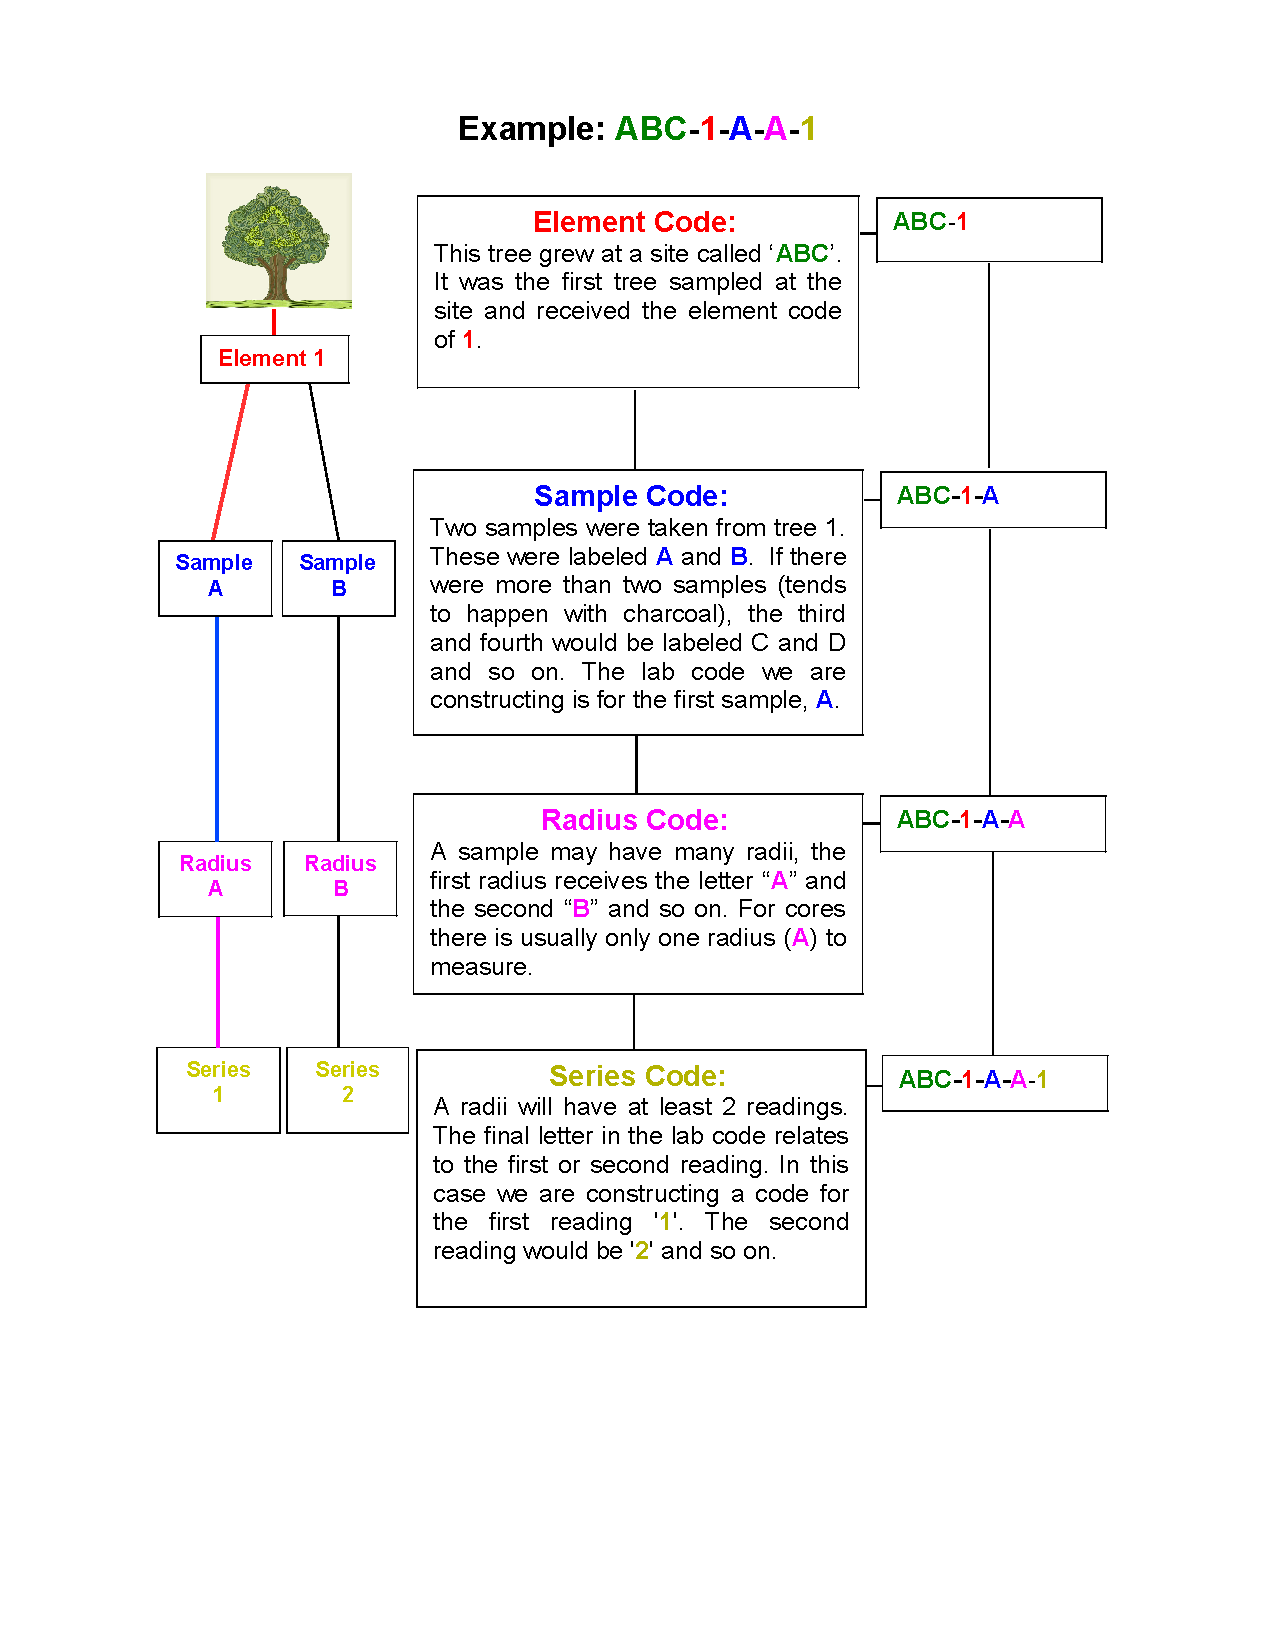
\includegraphics[trim = 1in 1.5in 1in 0.5in, clip, width=0.9\textwidth]{Images/CorinaSampleCodes.pdf}
\caption{Illustration of the how lab codes are built in Corina.  Figure courtesy of Charlotte Pearson.} 
\label{fig:labcodes}
\end{figure}

Lab codes are used throughout Corina to describe TRiDaS entities.  They can also be used in many places to specify entities that the user would like to choose.  For instance, in the database browser, you can type the lab code for an object, element, sample, radius or series to search the system for all the series that match the specified entity.  For instance entering `ABC-5' would search for all series associated with element `5' from object `ABC'.



\index{Metadata|)}


